
\documentclass[11pt,a4paper]{article}
\usepackage[utf8]{inputenc}
\usepackage{amsmath, amssymb, amsthm}
\usepackage{geometry}
\usepackage{graphicx} % Include graphics
\usepackage{hyperref} % Hyperlinks
\usepackage{enumerate} % Customizable enumeration
\geometry{a4paper, margin=1in}

\theoremstyle{plain}
\newtheorem{theorem}{Theorem}[section]
\newtheorem{lemma}[theorem]{Lemma}
\newtheorem{proposition}[theorem]{Proposition}
\newtheorem{corollary}[theorem]{Corollary}
\theoremstyle{definition}
\newtheorem{definition}[theorem]{Definition}
\newtheorem{example}[theorem]{Example}
\newtheorem*{definition*}{Definition}
\theoremstyle{remark}
\newtheorem*{remark}{Remark}
\newtheorem*{note}{Note}

\begin{document}

% \tableofcontents

\setcounter{section}{3} 
\section{Chapter 4}

We now move to briefly discuss Theorem 2, and the results in regards to compositionality and the complexity of deep networks, seeing how one might fit this to the discretisation that we have been discussing in the previous chapters.
This section will once again be a brief overview of \cite{Poggio}

\setcounter{theorem}{1} 
\begin{theorem}
    It considers a function \( f \in W_{m}^{2,n} \), the class of all compositional functions \(f\) of \(n\) variables with a binary tree architecture and constituent functions \(h\)  in \(W_{m}^{2}\)  and a deep network with a compositional architecture.\\
The activation function \( \sigma: \mathbb{R} \rightarrow \mathbb{R} \) in this context is also infinitely differentiable and not a polynomial. The complexity of the network necessary to provide an approximation with accuracy at least \( \varepsilon \) is 

\[ N = O((n - 1)\varepsilon^{-2/m}) \]
\end{theorem}

The above is taken as a particular case of a more general result, which we will now discuss. 

First we must define what we mean by a compositional function.

\begin{definition}[Compositional Function]
    We define  a compositional function in terms of a directed acyclic graph. 
    
    Let $\mathcal{G} $ be a directed acyclic graph (DAG), with the set of nodes $V$. We say \(f\) a \(\mathcal{G} \) function if
    \begin{itemize}
        \item Each of the source nodes obtains an input from $\mathbb{R}$.
        \item Each in-edge of every other node represents an input real variable, and the node itself represents a function of these input real variables, called a constituent function.
        \item The out-edges fan out the result of this evaluation. We assume that there is only one sink node, whose output is the $G$-function
    \end{itemize}
    If we were to ignore the compositionality of this function, it is a function of $n$ variables, where $n$ is the number of source nodes in $G$.
\end{definition}

\begin{theorem}[3]
    Let $\mathcal{G}$ be a DAG, $n$ be the number of source nodes, and for each $v \in V$, let $d_v$ be the number of in-edges of $v$. Let $f : \mathbb{R}^n \to \mathbb{R}$ be a compositional $\mathcal{G}$-function, where each of the constituent functions is in $W_{m_{v}}^{d_{v}}$. Consider shallow and deep networks with infinitely smooth activation function as in Theorem 1. Then deep networks – with an associated graph that corresponds to the graph of $f$ – avoid the curse of dimensionality in approximating $f$ for increasing $n$, whereas shallow networks cannot directly avoid the curse. In particular, the complexity of the best approximating shallow network is exponential in $n$
    \[
        N_s = \mathcal{O}\left(\epsilon^{-\frac{n}{m}}\right),
    \]
    where $m = \min_{v \in V} m_v$, while the complexity of the deep network is
    \[
        N_d = \mathcal{O}\left(\sum_{v \in V} \epsilon^{-\frac{d_v}{m_v}}\right).
    \]
    We call $\frac{d_v}{m_v}$ the \textbf{effective dimension} of function $v$. Then, deep networks can avoid the curse of dimensionality if the constituent functions of a compositional function have a small effective dimension; i.e., have fixed, “small” dimensionality or fixed, “small” “roughness”.
\end{theorem}

\begin{example}
    We discuss an example already seen in the previous chapter, where we consider the function $Q(x, y) = |x^{2}  - y^{2}|$ and the associated graph $\mathcal{G}$, and the associated deep network. 

    Here we expect this continuous function of 2 variables to have an effective dimension of 2, and hence, a shallow network would require at least \(c \epsilon^{-2} \) parameters to approximate it within \(\epsilon \). However we can exploit the compositional structure of the function to construct a deep network with a much smaller number of parameters, as we have seen in the previous chapter. The diagrams below show how the deep network can be constructed from the graph of the function, considering each of its constituent functions - we see they both have effective dimensions of 1. We should hence be able to construct a 2-layer deep network with \(c \epsilon^{-1} \) parameters to approximate the function within \(\epsilon \).
    
    \begin{figure}[h]
        \centering
        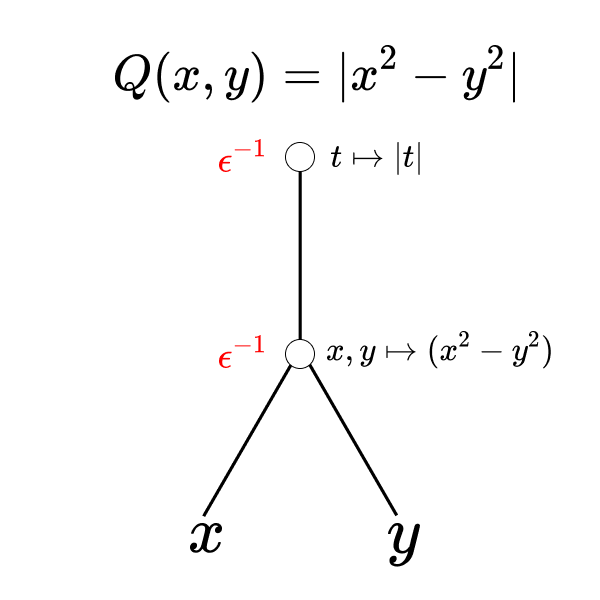
\includegraphics[width=0.45\textwidth]{diags/Comp.png}
        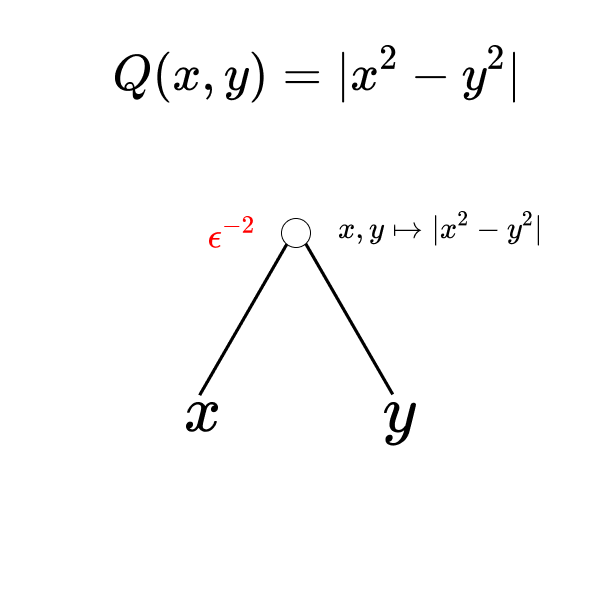
\includegraphics[width=0.45\textwidth]{diags/CompShallow.png}
        \caption{Compositional Structures}
    \end{figure}
    
    \begin{figure}[h]
        \centering
        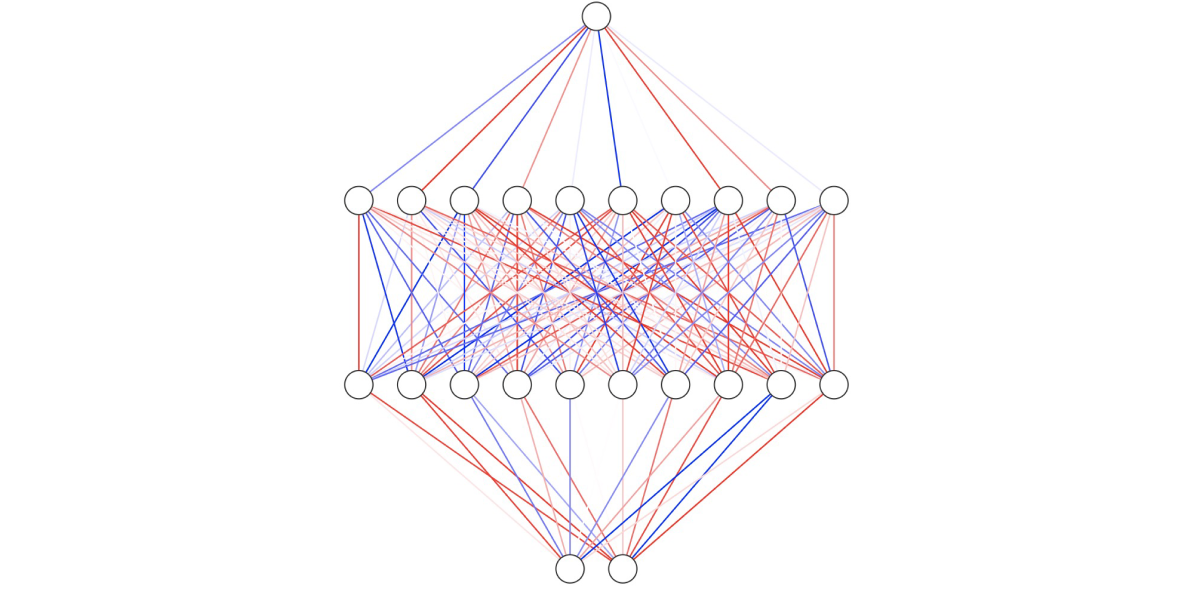
\includegraphics[width=0.49\textwidth]{diags/DeepQ.png}
        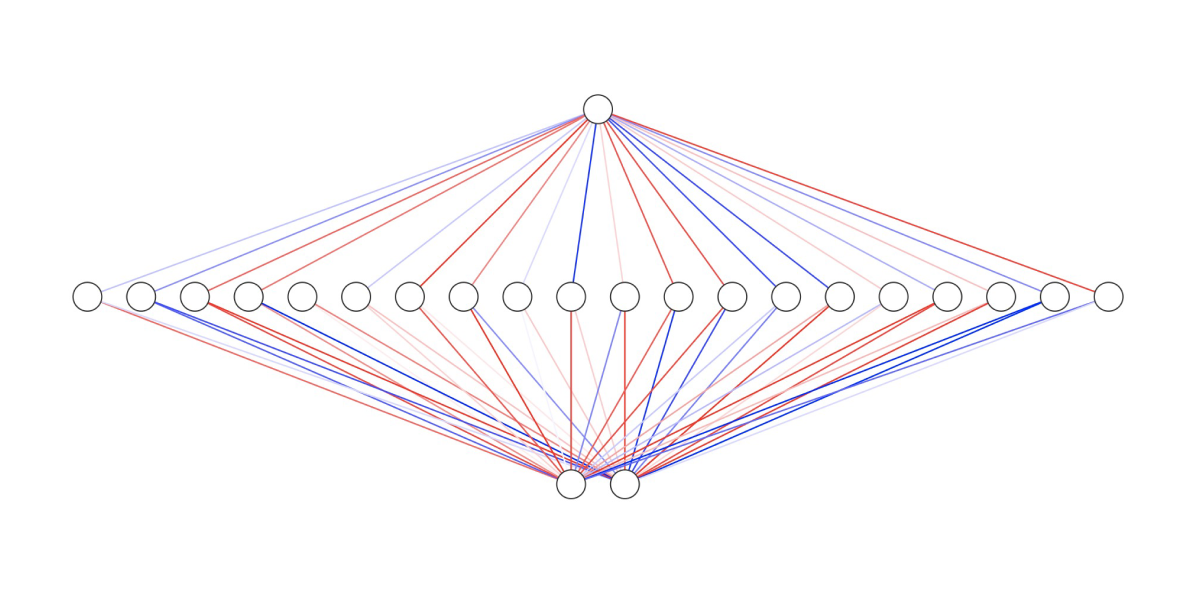
\includegraphics[width=0.49\textwidth]{diags/ShallowQ.png}
        \caption{Corresponding Deep and Shallow Networks}
    \end{figure}
    
\end{example}

We aim to run tests for the following examples to see how well the theoretical results hold up in practice, and how we can adapt them to our discretised framework.

\begin{enumerate}
    \item The function $Q(x, y) = |x^{2}  - y^{2}|$ and the associated deep network.
    \item The function $h_2(h_{11}(x_1,x_2), h_{12}(x_3,x_4)) = \sqrt{4 \cdot (2x_1 + 4x_2)^4 + 5 \cdot (2x_3 + 3x_4)^4}$ and the associated binary tree network.
\end{enumerate}

Within my code - I have implemented the following classes: \verb|BinaryNetwork|, which creates a binary tree network, and \verb|DeepNetwork|, which creates a deep network.
The binary network is simply constructed by passing in the number of leaves of the tree for some \(2^k\) and an associated number of neurons for each node in the tree. 
The deep network is constructed by passing a DAG (Directed Acylcic Graph) and a list of neurons for each node in the graph, representing the effective dimension of the component functions of our compositional target function.

\begin{figure}[h]
    \centering
    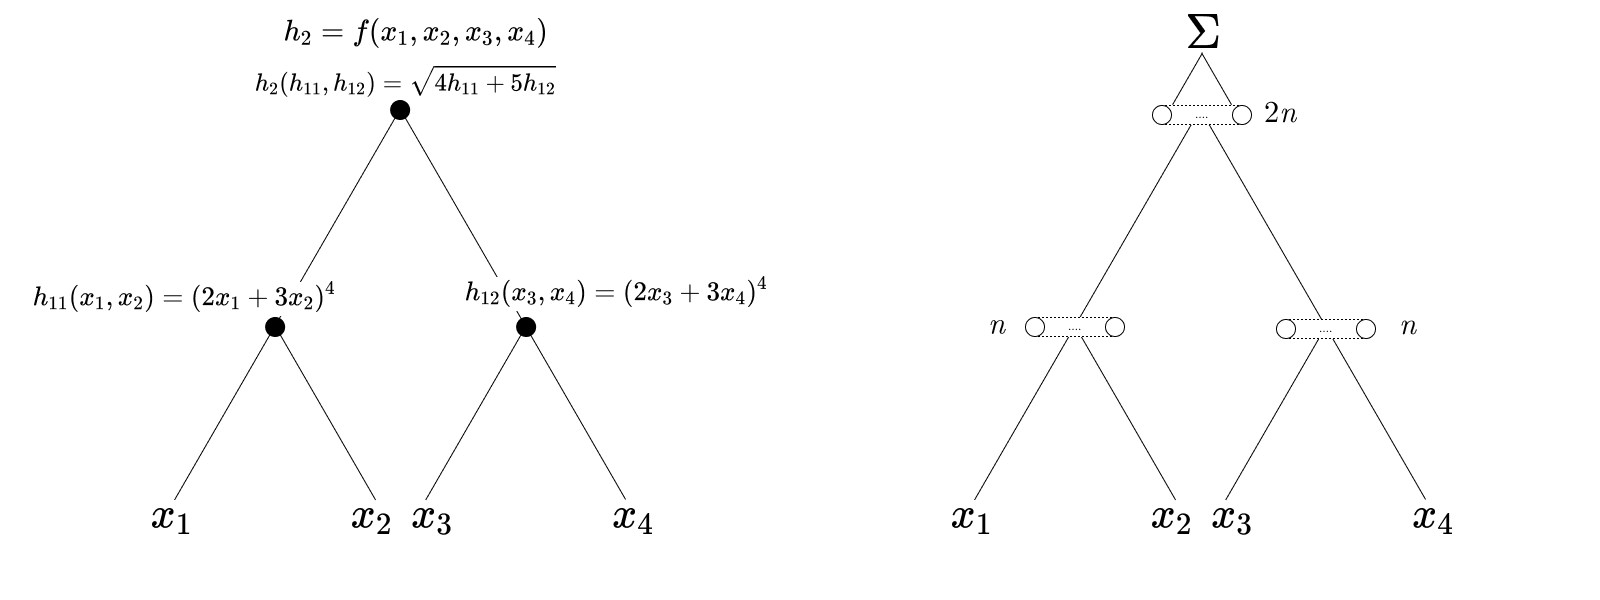
\includegraphics[width=\textwidth]{diags/BinaryTree.png}
    \caption{Compositional structure of \(h\) and associated binary tree network}
    \label{fig:}
\end{figure}

We use \(Q\) and \(h\) as our target functions, and we aim to approximate them using the binary tree and deep networks respectively. We will then make the comparison between the number of parameters required to approximate the function within a given \(\epsilon \) for both the deep and shallow networks, and see how well the theoretical results hold up in practice.


\end{document}